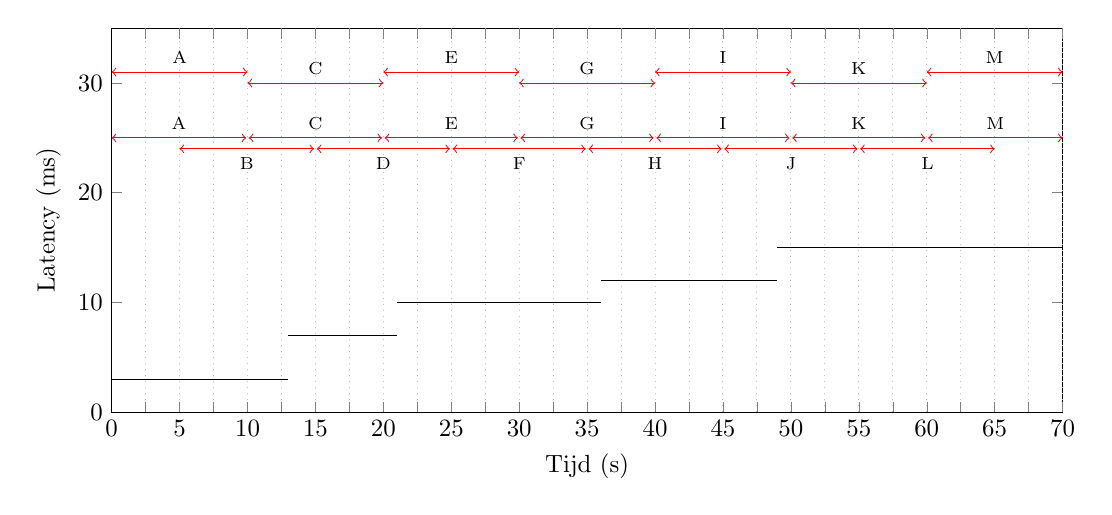
\begin{tikzpicture}[scale=0.9]
\begin{axis}[
xlabel={Tijd (s)},
ylabel={Latency (ms)},
xmin=0,xmax=70,
ymin=0,ymax=35,
legend style={
	cells={anchor=west},
	legend pos=outer north east,
},
extra x ticks ={2.5,5,7.5,...,70},
extra x tick labels={,,,},
extra x tick style={grid=major, grid style={dotted}},
width = 15cm,
height = 7cm
]



after end axis/.code={
	\draw (axis cs:0,3) -- (axis cs:13,3);
	\draw (axis cs:13,7) -- (axis cs:21,7);
	\draw (axis cs:21,10) -- (axis cs:36,10);
	\draw (axis cs:36,12) -- (axis cs:49,12);
	\draw (axis cs:49,15) -- (axis cs:70,15);
	
	\draw[red,<->] (axis cs:0,31) -- (axis cs:10,31)	node [pos=0.5,above,font=\scriptsize,color=black] {A};
	\draw[red,<->] (axis cs:10,30) -- (axis cs:20,30)	node [pos=0.5,above,font=\scriptsize,color=black] {C};
	\draw[red,<->] (axis cs:20,31) -- (axis cs:30,31)	node [pos=0.5,above,font=\scriptsize,color=black] {E};
	\draw[red,<->] (axis cs:30,30) -- (axis cs:40,30)	node [pos=0.5,above,font=\scriptsize,color=black] {G};
	\draw[red,<->] (axis cs:40,31) -- (axis cs:50,31)	node [pos=0.5,above,font=\scriptsize,color=black] {I};
	\draw[red,<->] (axis cs:50,30) -- (axis cs:60,30)	node [pos=0.5,above,font=\scriptsize,color=black] {K};
	\draw[red,<->] (axis cs:60,31) -- (axis cs:70,31)	node [pos=0.5,above,font=\scriptsize,color=black] {M};
	
	\draw[red,<->] (axis cs:0,25) -- (axis cs:9.9,25)	node [pos=0.5,above,font=\scriptsize,color=black] {A};
	\draw[red,<->] (axis cs:5,24) -- (axis cs:14.9,24)	node [pos=0.5,below,font=\scriptsize,color=black] {B};
	\draw[red,<->] (axis cs:10.1,25) -- (axis cs:19.9,25)	node [pos=0.5,above,font=\scriptsize,color=black] {C};
	\draw[red,<->] (axis cs:15.1,24) -- (axis cs:24.9,24)	node [pos=0.5,below,font=\scriptsize,color=black] {D};
	\draw[red,<->] (axis cs:20.1,25) -- (axis cs:29.9,25)	node [pos=0.5,above,font=\scriptsize,color=black] {E};
	\draw[red,<->] (axis cs:25.1,24) -- (axis cs:34.9,24)	node [pos=0.5,below,font=\scriptsize,color=black] {F};
	\draw[red,<->] (axis cs:30.1,25) -- (axis cs:39.9,25)	node [pos=0.5,above,font=\scriptsize,color=black] {G};
	\draw[red,<->] (axis cs:35.1,24) -- (axis cs:44.9,24)	node [pos=0.5,below,font=\scriptsize,color=black] {H};
	\draw[red,<->] (axis cs:40.1,25) -- (axis cs:49.9,25)	node [pos=0.5,above,font=\scriptsize,color=black] {I};
	\draw[red,<->] (axis cs:45.1,24) -- (axis cs:54.9,24)	node [pos=0.5,below,font=\scriptsize,color=black] {J};
	\draw[red,<->] (axis cs:50.1,25) -- (axis cs:59.9,25)	node [pos=0.5,above,font=\scriptsize,color=black] {K};
	\draw[red,<->] (axis cs:55.1,24) -- (axis cs:65,24)	node [pos=0.5,below,font=\scriptsize,color=black] {L};
	\draw[red,<->] (axis cs:60.1,25) -- (axis cs:70,25)	node [pos=0.5,above,font=\scriptsize,color=black] {M};
	
%	\draw[black,<->] (axis cs:10,0.2) -- (axis cs:20,0.2)	node [pos=0.5,above,font=\scriptsize] {buffer $i$};
	
%	\draw[black,<->] (axis cs:20,0.3) -- (axis cs:30,0.3)	node [pos=0.5,above,font=\scriptsize] {buffer $i+1$};
}]

\end{axis}

\end{tikzpicture}